\documentclass[12pt, a4paper, oneside]{article}
\usepackage{amsmath, amsthm, amssymb, appendix, bm, graphicx, hyperref, mathrsfs, makecell}
\usepackage{bbm, stfloats, subfigure, pythonhighlight, CJK, algorithm, algorithmicx, algpseudocode}
\usepackage{geometry}
\geometry{a4paper,left=2.5cm,right=2.5cm,top=3cm,bottom=3cm}
\usepackage{fancyhdr}
\pagestyle{fancy}
\renewcommand\headrulewidth{.5pt}
\renewcommand\footrulewidth{0pt}
\setlength{\headheight}{15pt}
\fancyhead[L]{\textit{\leftmark}}
\fancyhead[R]{\thepage}

\title{\textbf{Federated CP New Setting}}
\author{Min, Xia}
\date{\today}
\linespread{1.6}
\definecolor{lightBlue}{rgb}{0.274,0.41,0.879}
\definecolor{darckGreen}{rgb}{0.1797,0.543,0.3398}
%{\color{lightBlue}Text Here}
\newtheorem{theorem}{Theorem}[section]
\newtheorem{definition}[theorem]{Definition}
\newtheorem{lemma}[theorem]{Lemma}
\newtheorem{corollary}[theorem]{Corollary}
\newtheorem{example}[theorem]{Example}
\newtheorem{proposition}[theorem]{Proposition}
\newtheorem{remark}[theorem]{Remark}
\renewcommand{\abstractname}{\Large\textbf{Abstract}}
\floatname{algorithm}{Algorithm}
\renewcommand{\algorithmicrequire}{\textbf{Input:}}
\renewcommand{\algorithmicensure}{\textbf{Output:}}

\begin{document}
\maketitle
\setcounter{page}{1}
\pagenumbering{arabic}
\section{Idea1}
    For $K$ agents each with $Z_k=\{(X_i^k,Y_i^k)\}_{i=1}^{n_k}$ sampled from distribution $P^k$, and point predictor $f_1$ based score $S_i^k$. If all $P^k=P$ and a new test point $X,Y$ from $P^1$. For any trial data $y$ and score $S$ follow the procedure in "Conformal prediction with local weights: randomization enables robust guarantees"\cite{hore2023conformal}:
    \begin{itemize}
        \item Find some kernel function $H(\cdot,\cdot)$, sample $\tilde{X}$ based on $H(X,\cdot)$.
        \item Calculate empirical function $\tilde{F}=\overset{}{\underset{i,k}\sum}w_i^k\delta_{S_i^k}+w\delta_{S}$ with weight
        \begin{equation*}
            w_i^k=\dfrac{H(X_i^k,\tilde{X})}{\overset{}{\underset{i',k'}\sum}H(X_{i'}^{k'},\tilde{X})+H(X,\tilde{X})},\ w=\dfrac{H(X,\tilde{X})}{\overset{}{\underset{i',k'}\sum}H(X_{i'}^{k'},\tilde{X})+H(X,\tilde{X})}.
        \end{equation*}
        \item Conformal set is $C_\alpha(X)=\{S\leq Q(1-\alpha,\tilde{F})\}$.
    \end{itemize}


    However for all $k$ $P^k=P$ is not practical, potential covariate shift exists

\subsection{Experiment1}
    Assume agent $k=1,\cdots,K$ each has $n$ samples $X_1^k,\cdots,X_n^k$ follow $N(\mu_k,9)$. Sythesize $Y_i^k=(X_i^k)^2+\epsilon$, where $\epsilon\sim N(0,(ep*|X|)^2)$, $ep$ be some parameter. Under this problem only have covariate shift.

    \begin{itemize}
        \item $X$ has different distribution for each agents
        \item $EY|X$ is same for all agents
        \item $Y-EY|X$ has same distribution for all agents
    \end{itemize}
    

    Covariate shift has little influence on this method as the method is localized. More on Fig \ref{Fig1}.
    \begin{figure}[htbp]
        \centering
        \begin{minipage}{0.495\linewidth}
            \centering
            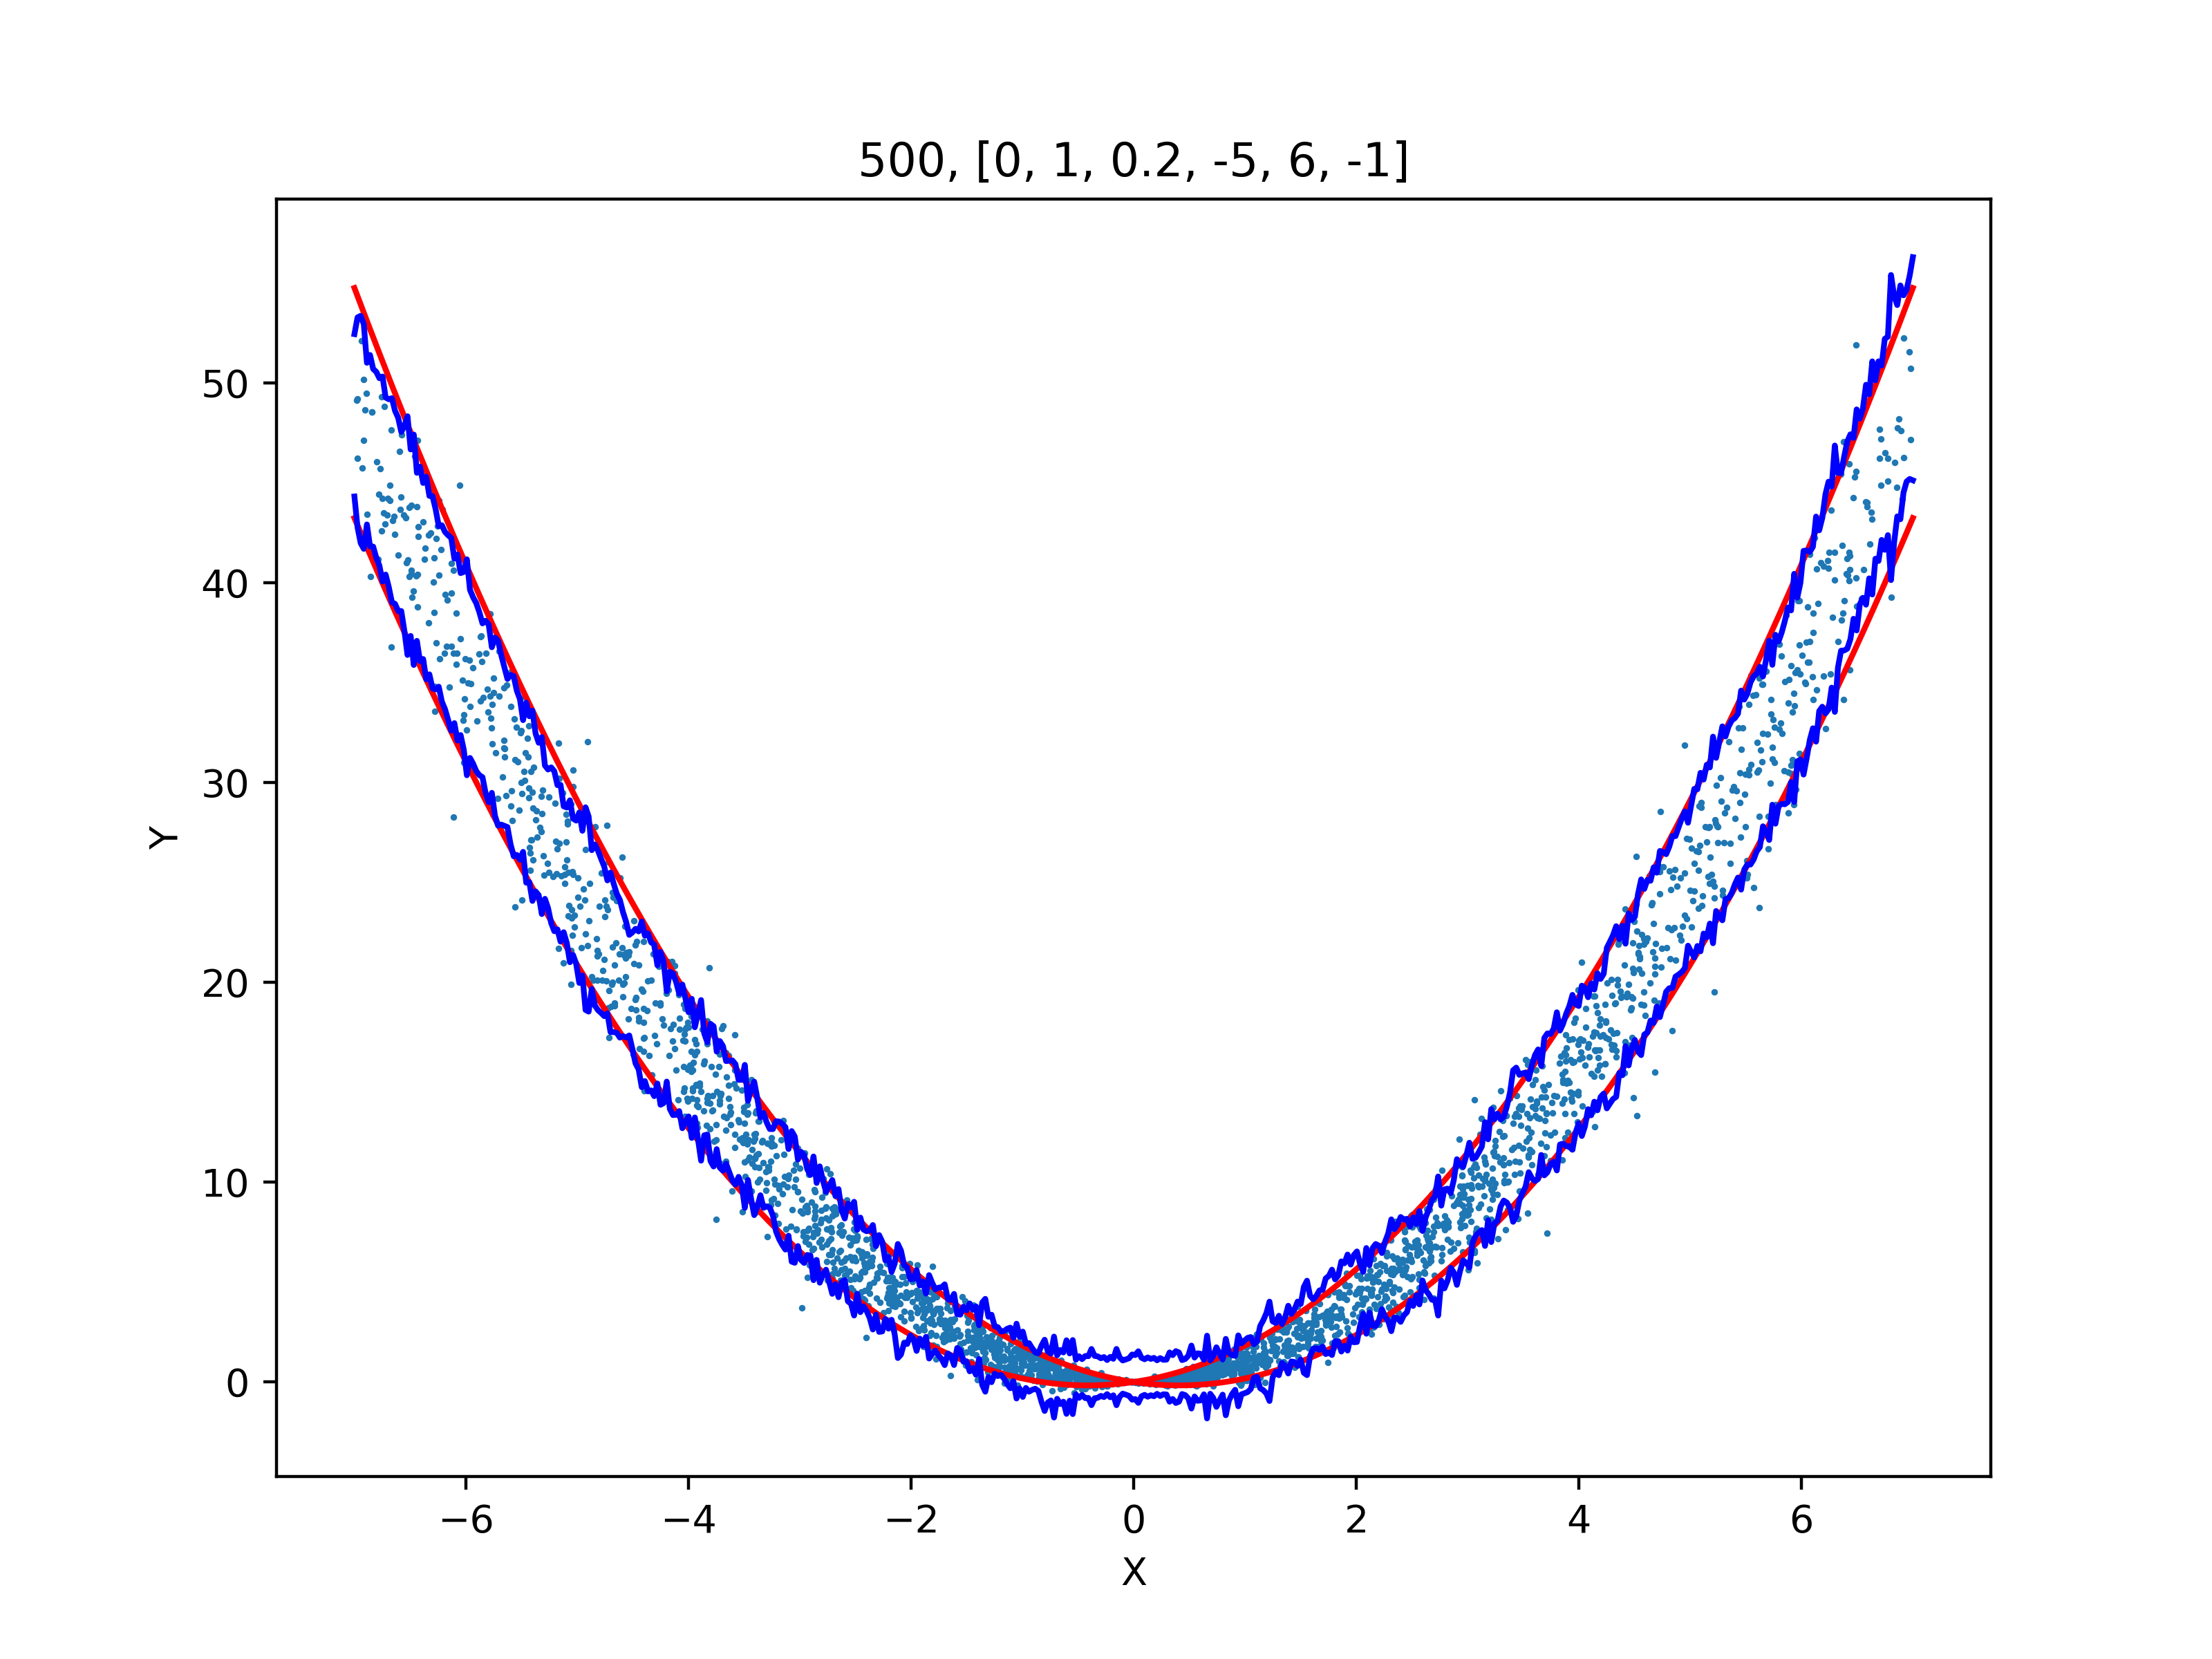
\includegraphics[width=0.98\linewidth]{fig/Ex1_1/0_1_.png}
        \end{minipage}
        \begin{minipage}{0.495\linewidth}
            \centering
            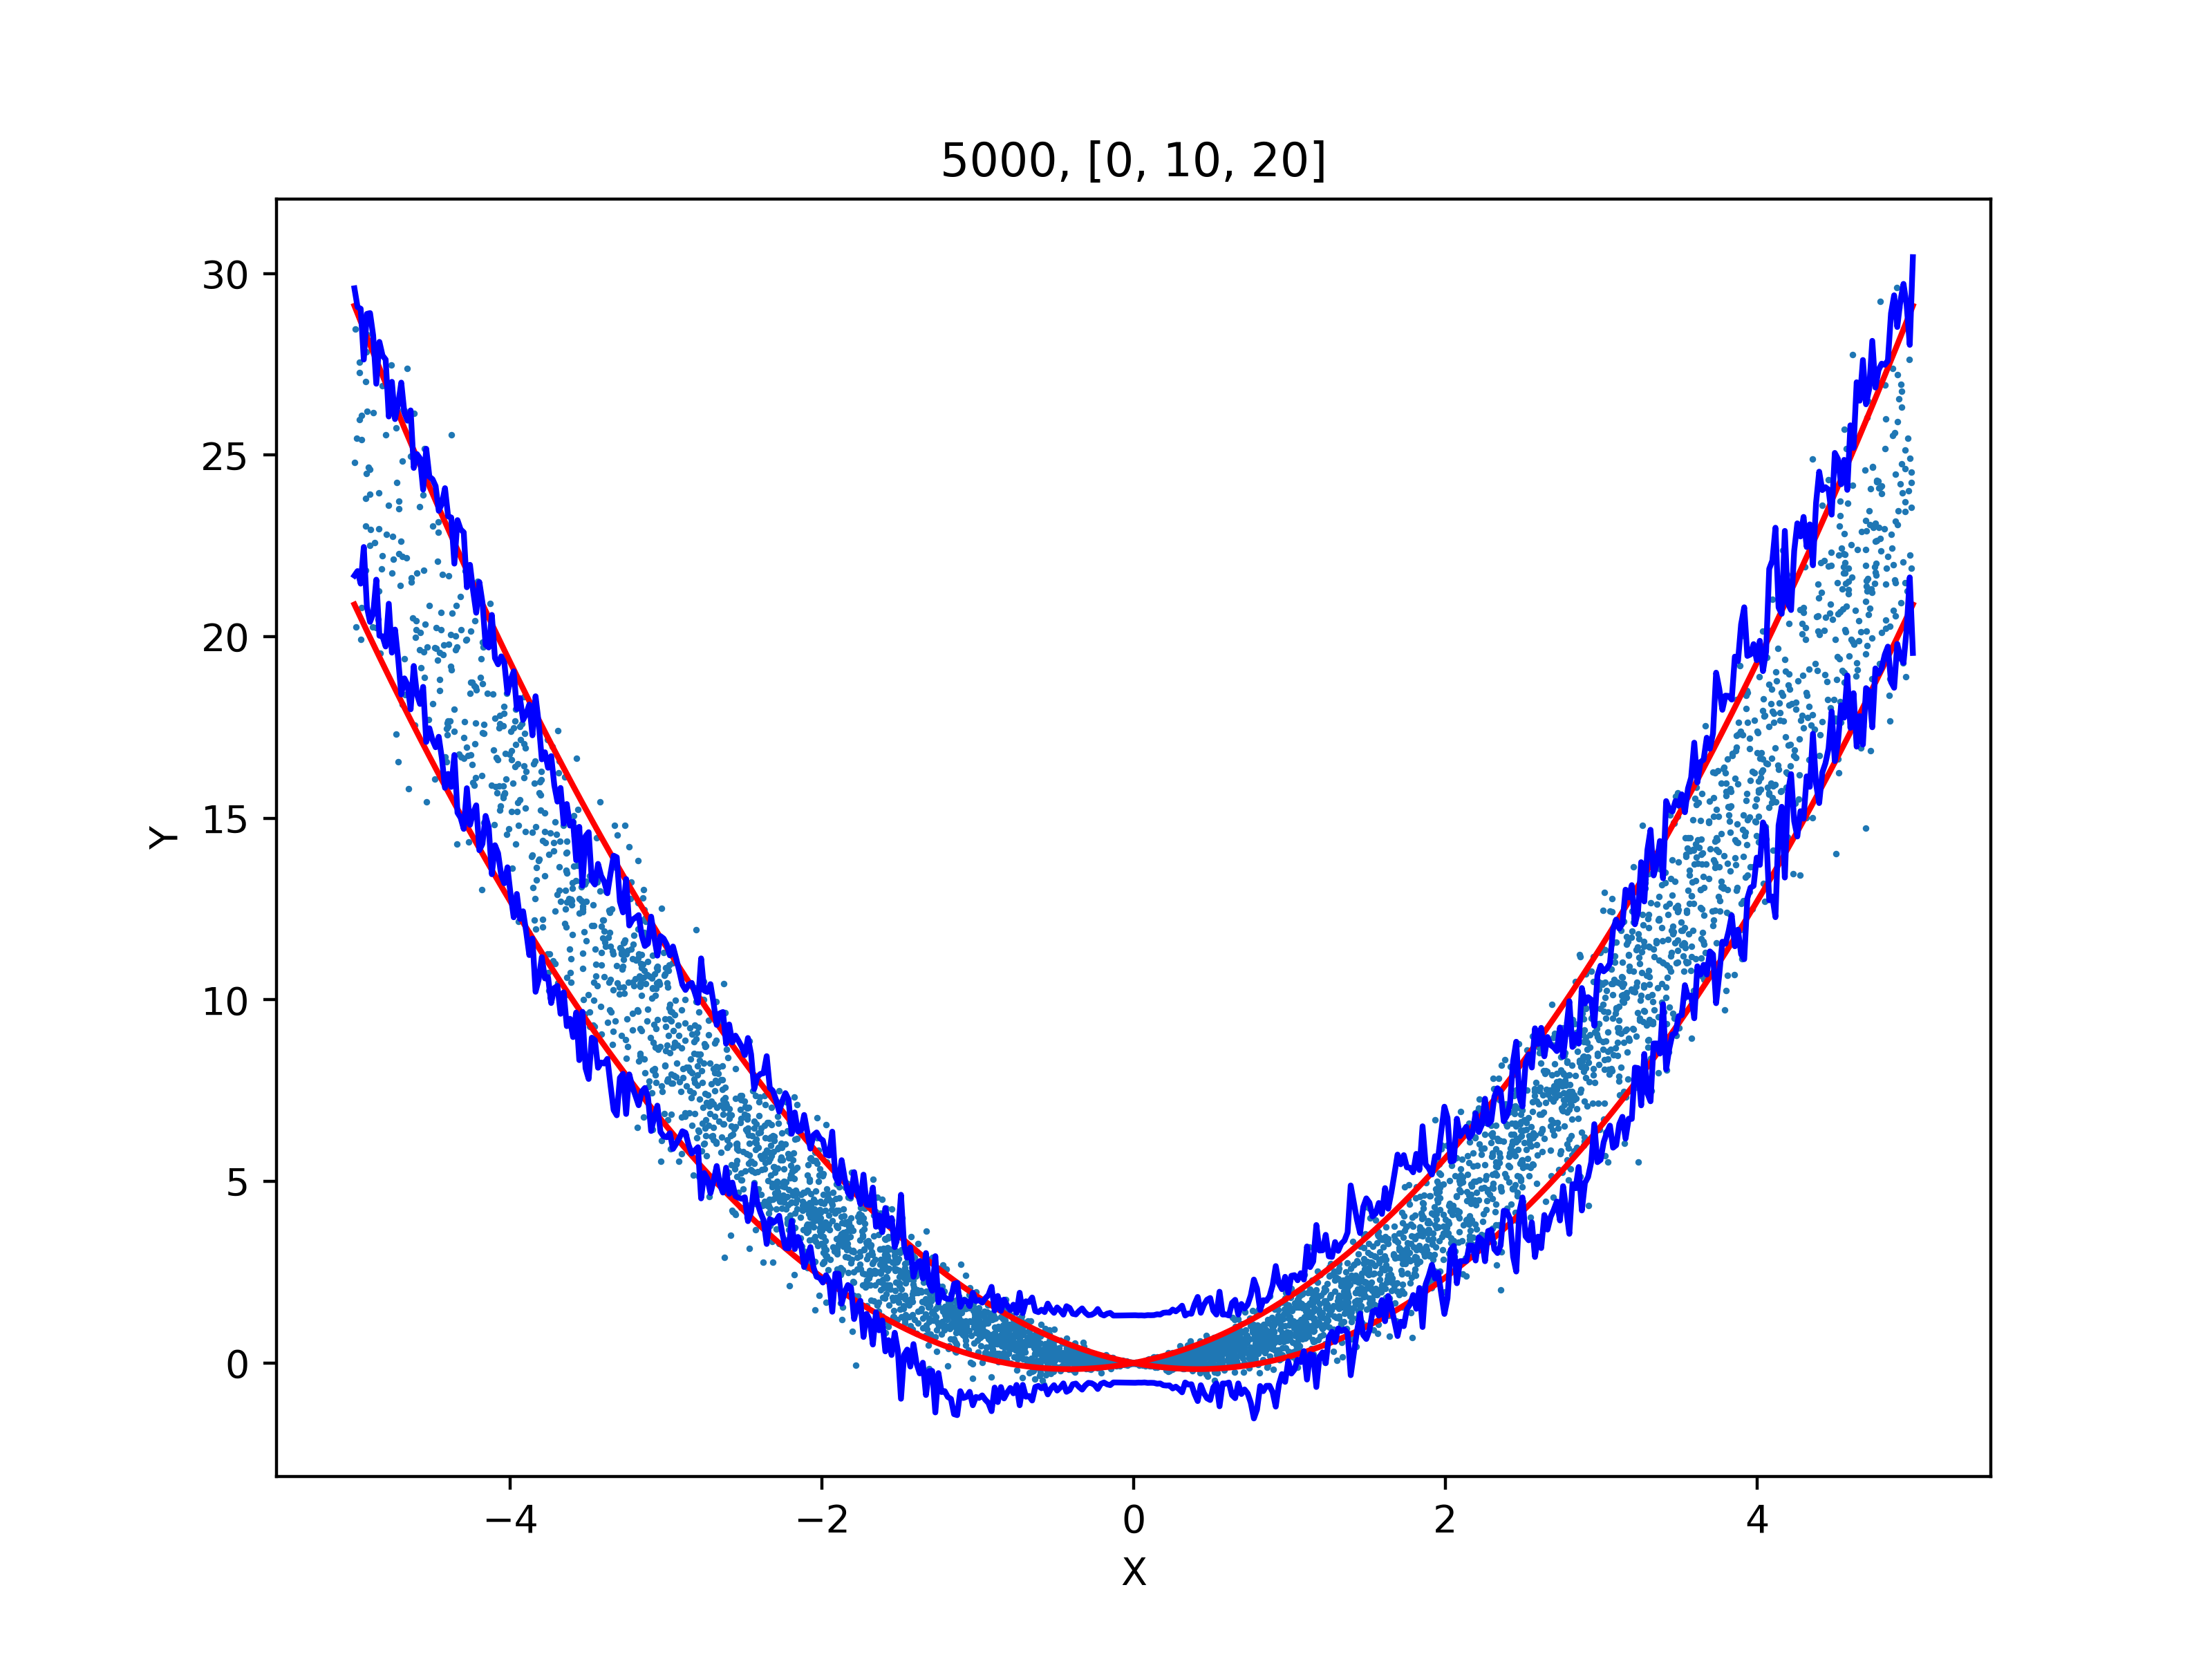
\includegraphics[width=0.98\linewidth]{fig/Ex1_1/0_10_20.png}
        \end{minipage}
        \centering
        \begin{minipage}{0.495\linewidth}
            \centering
            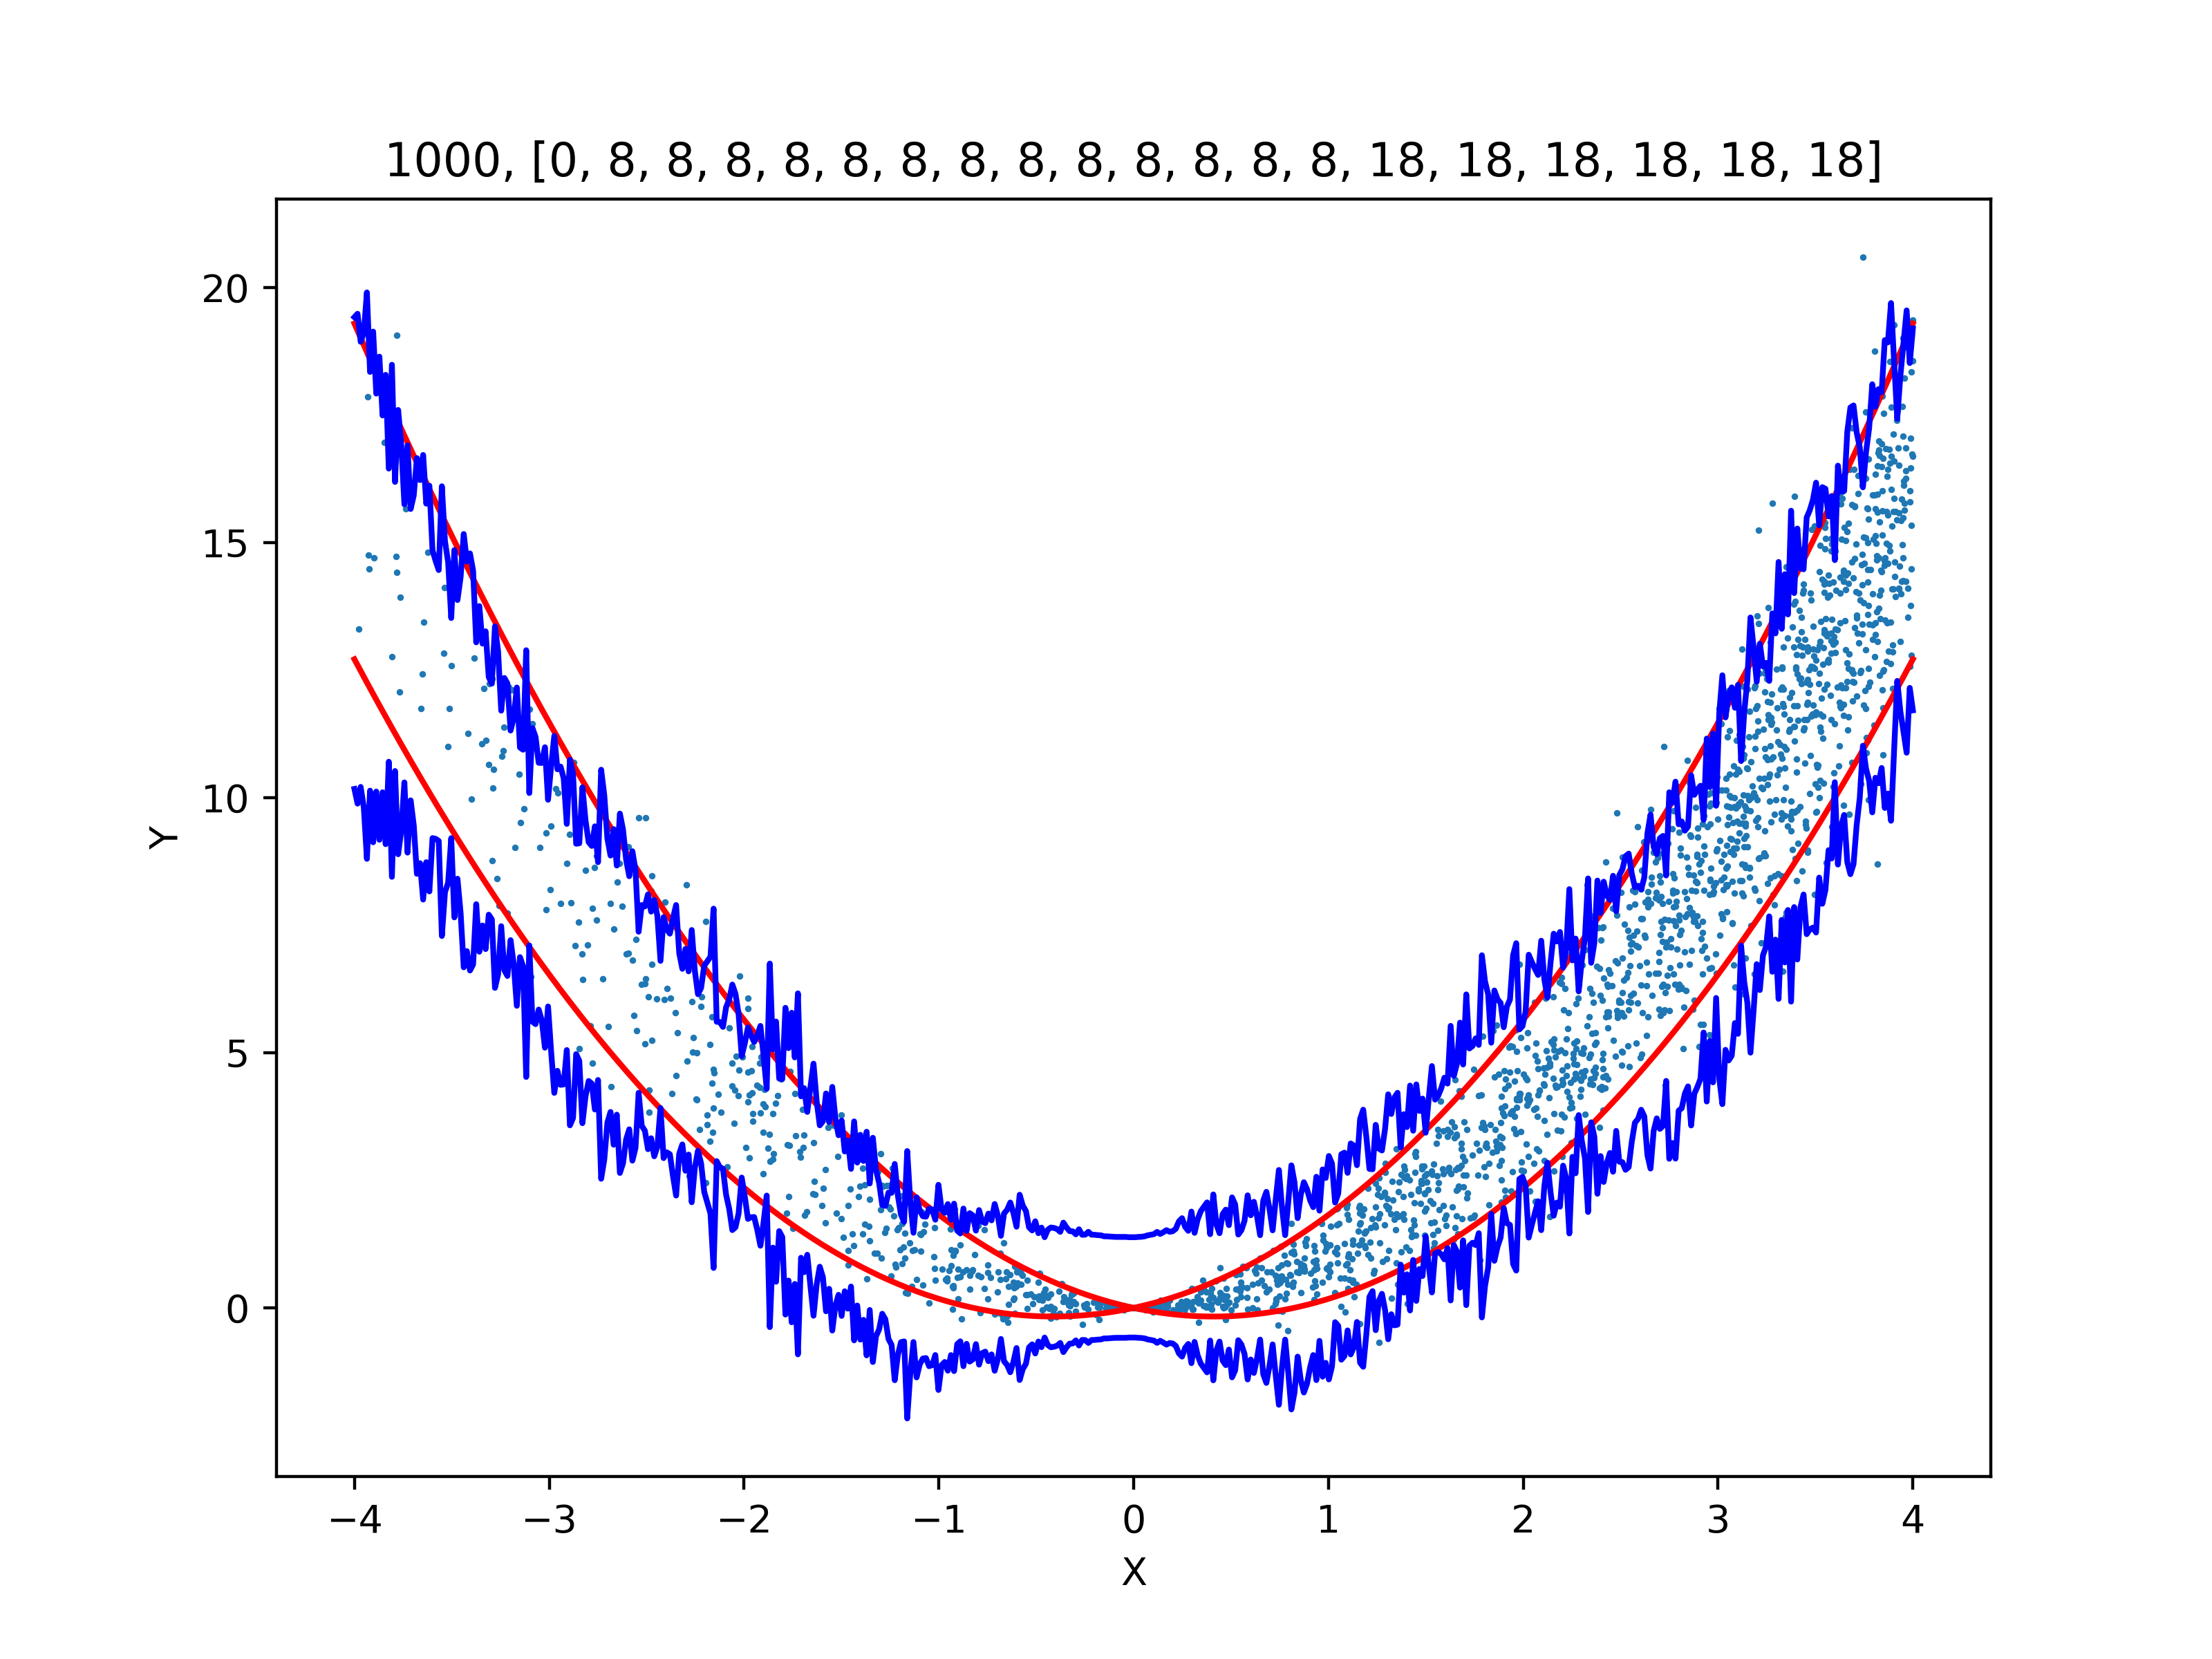
\includegraphics[width=0.98\linewidth]{fig/Ex1_1/0_8_18.png}
        \end{minipage}
        \begin{minipage}{0.495\linewidth}
            \centering
            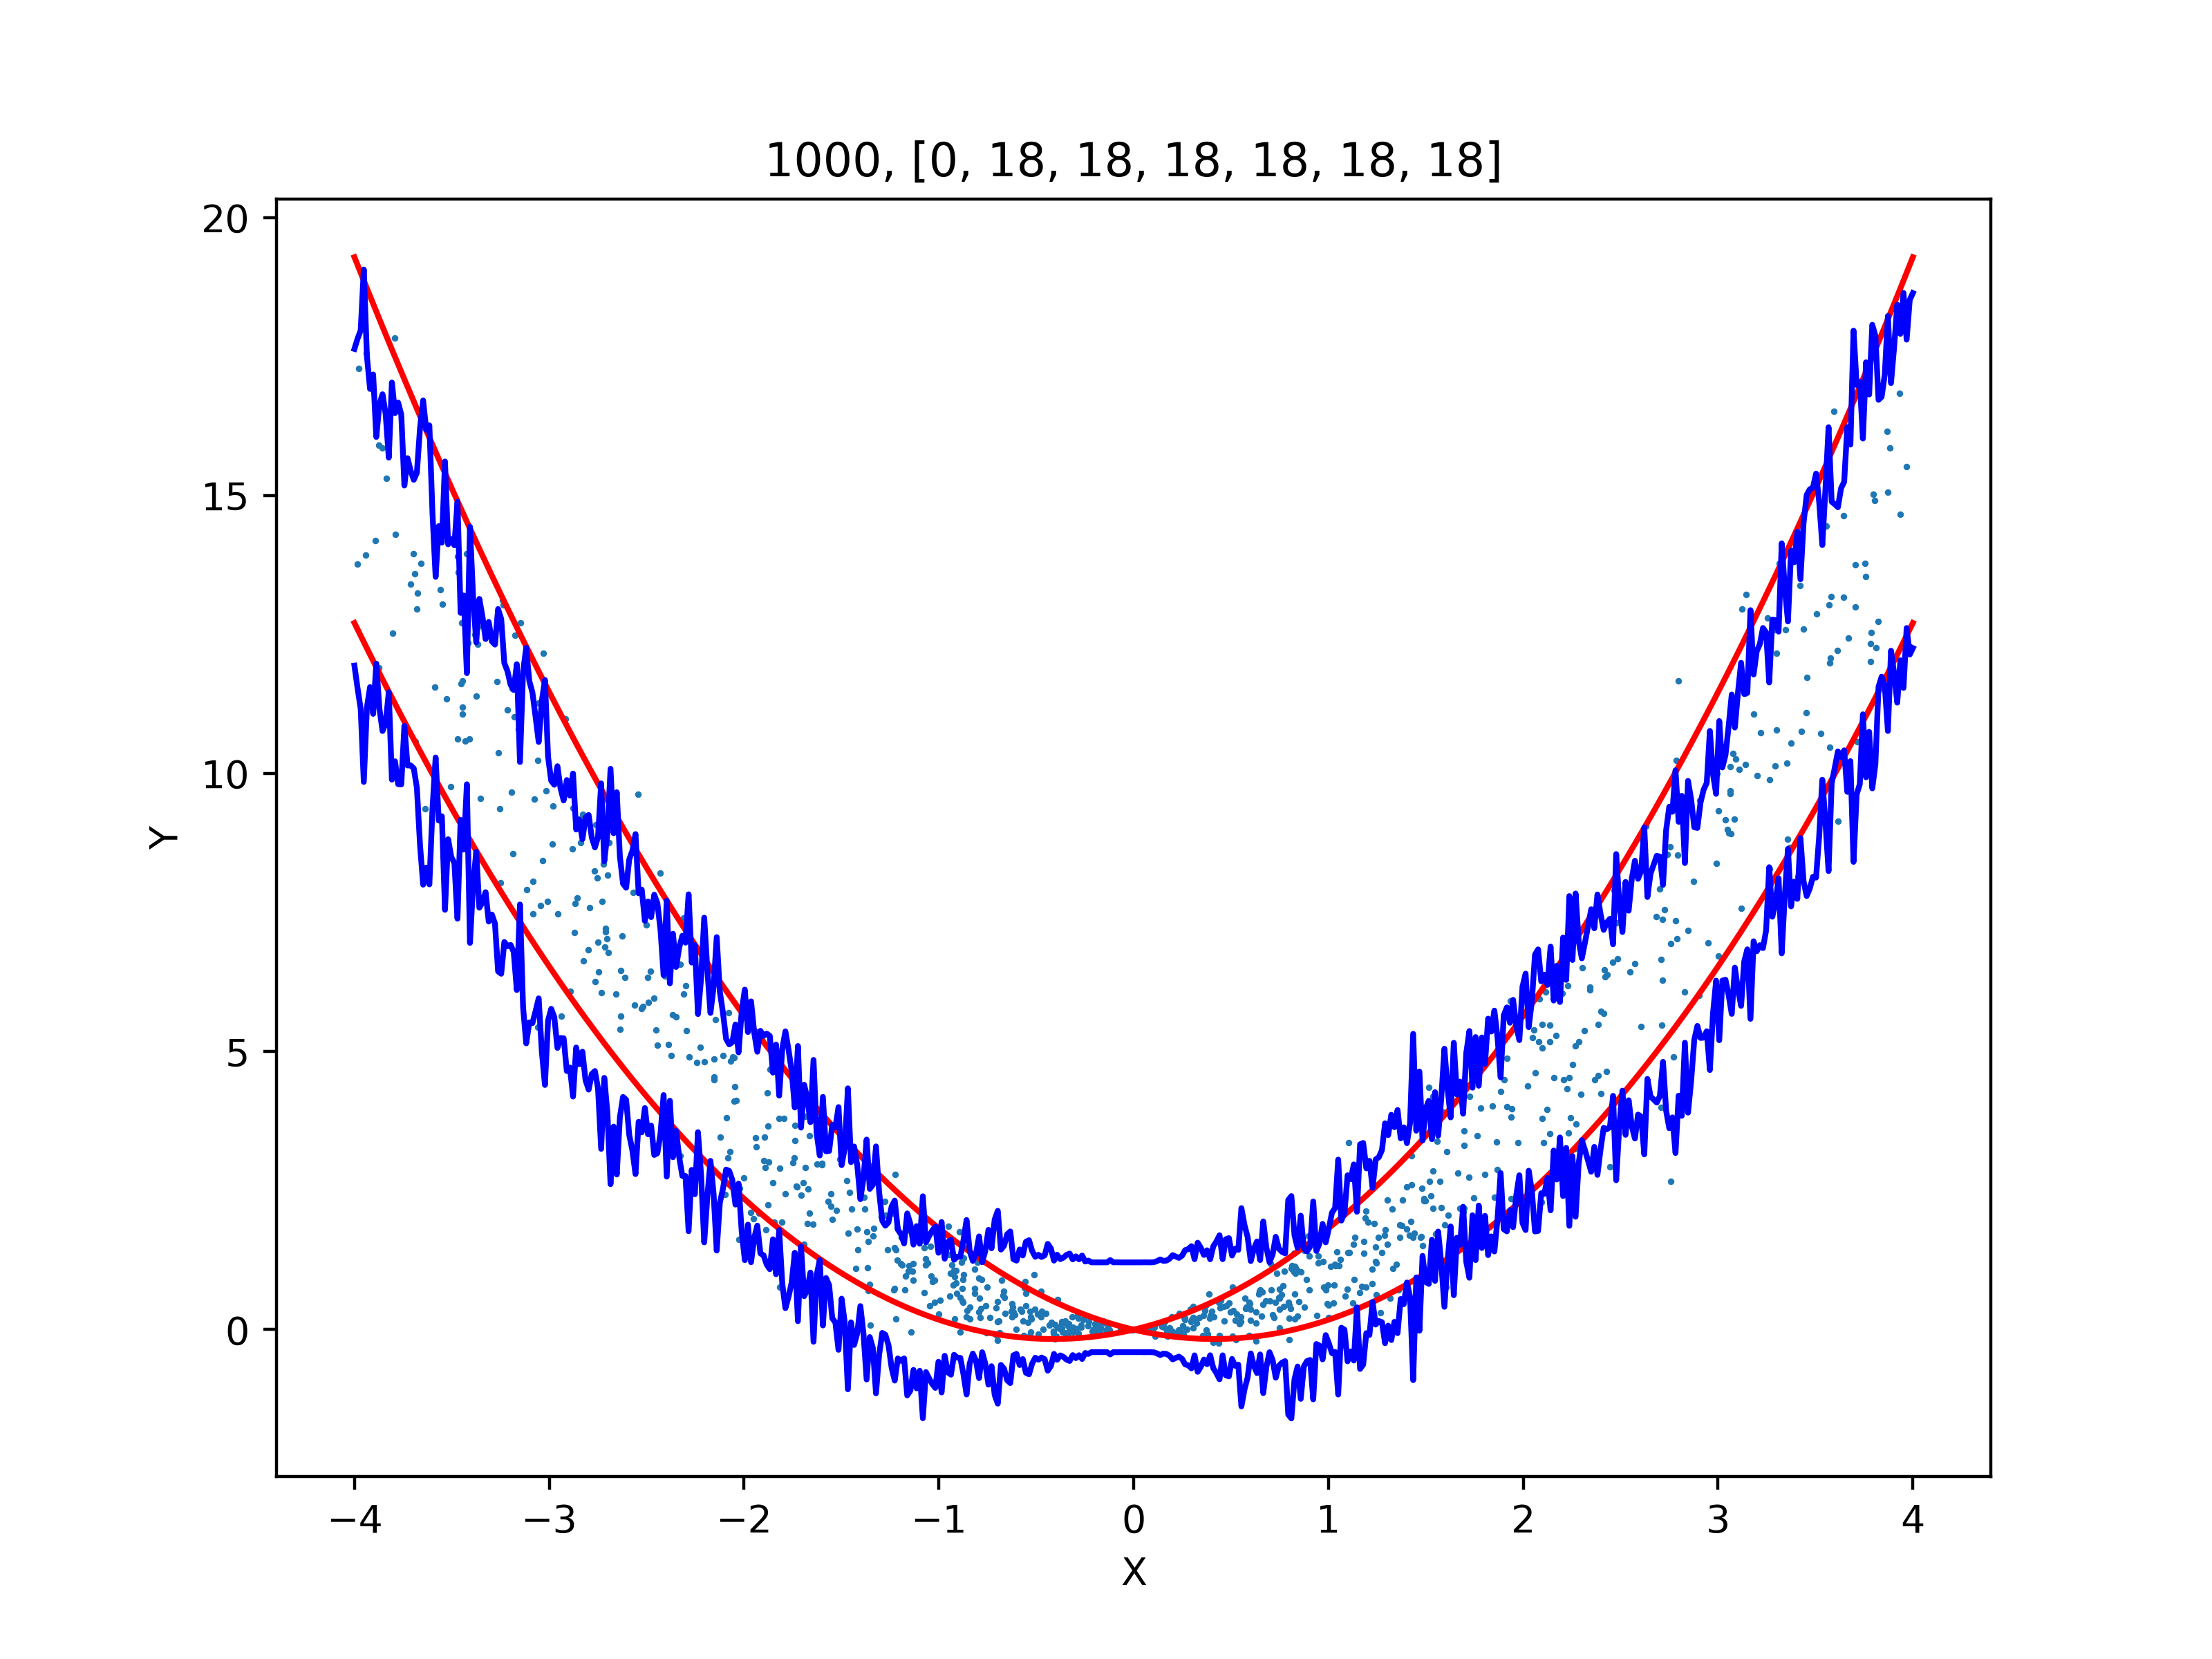
\includegraphics[width=0.98\linewidth]{fig/Ex1_1/0_18.png}
        \end{minipage}
        \caption{Fig1}
        \label{Fig1}
    \end{figure}

    Generate 1000 samples with location 0, and 1000 samples with location 0 and 20. The left shows the performance on only within samples with 0 location and 1000 samples is better than the right one using 2000 data samples. This comes from covariate shift, the scores from samples with location 20 influences origin behavior, from Fig \ref{Fig2}
    \begin{figure}[htbp]
        \centering
        \begin{minipage}{0.495\linewidth}
            \centering
            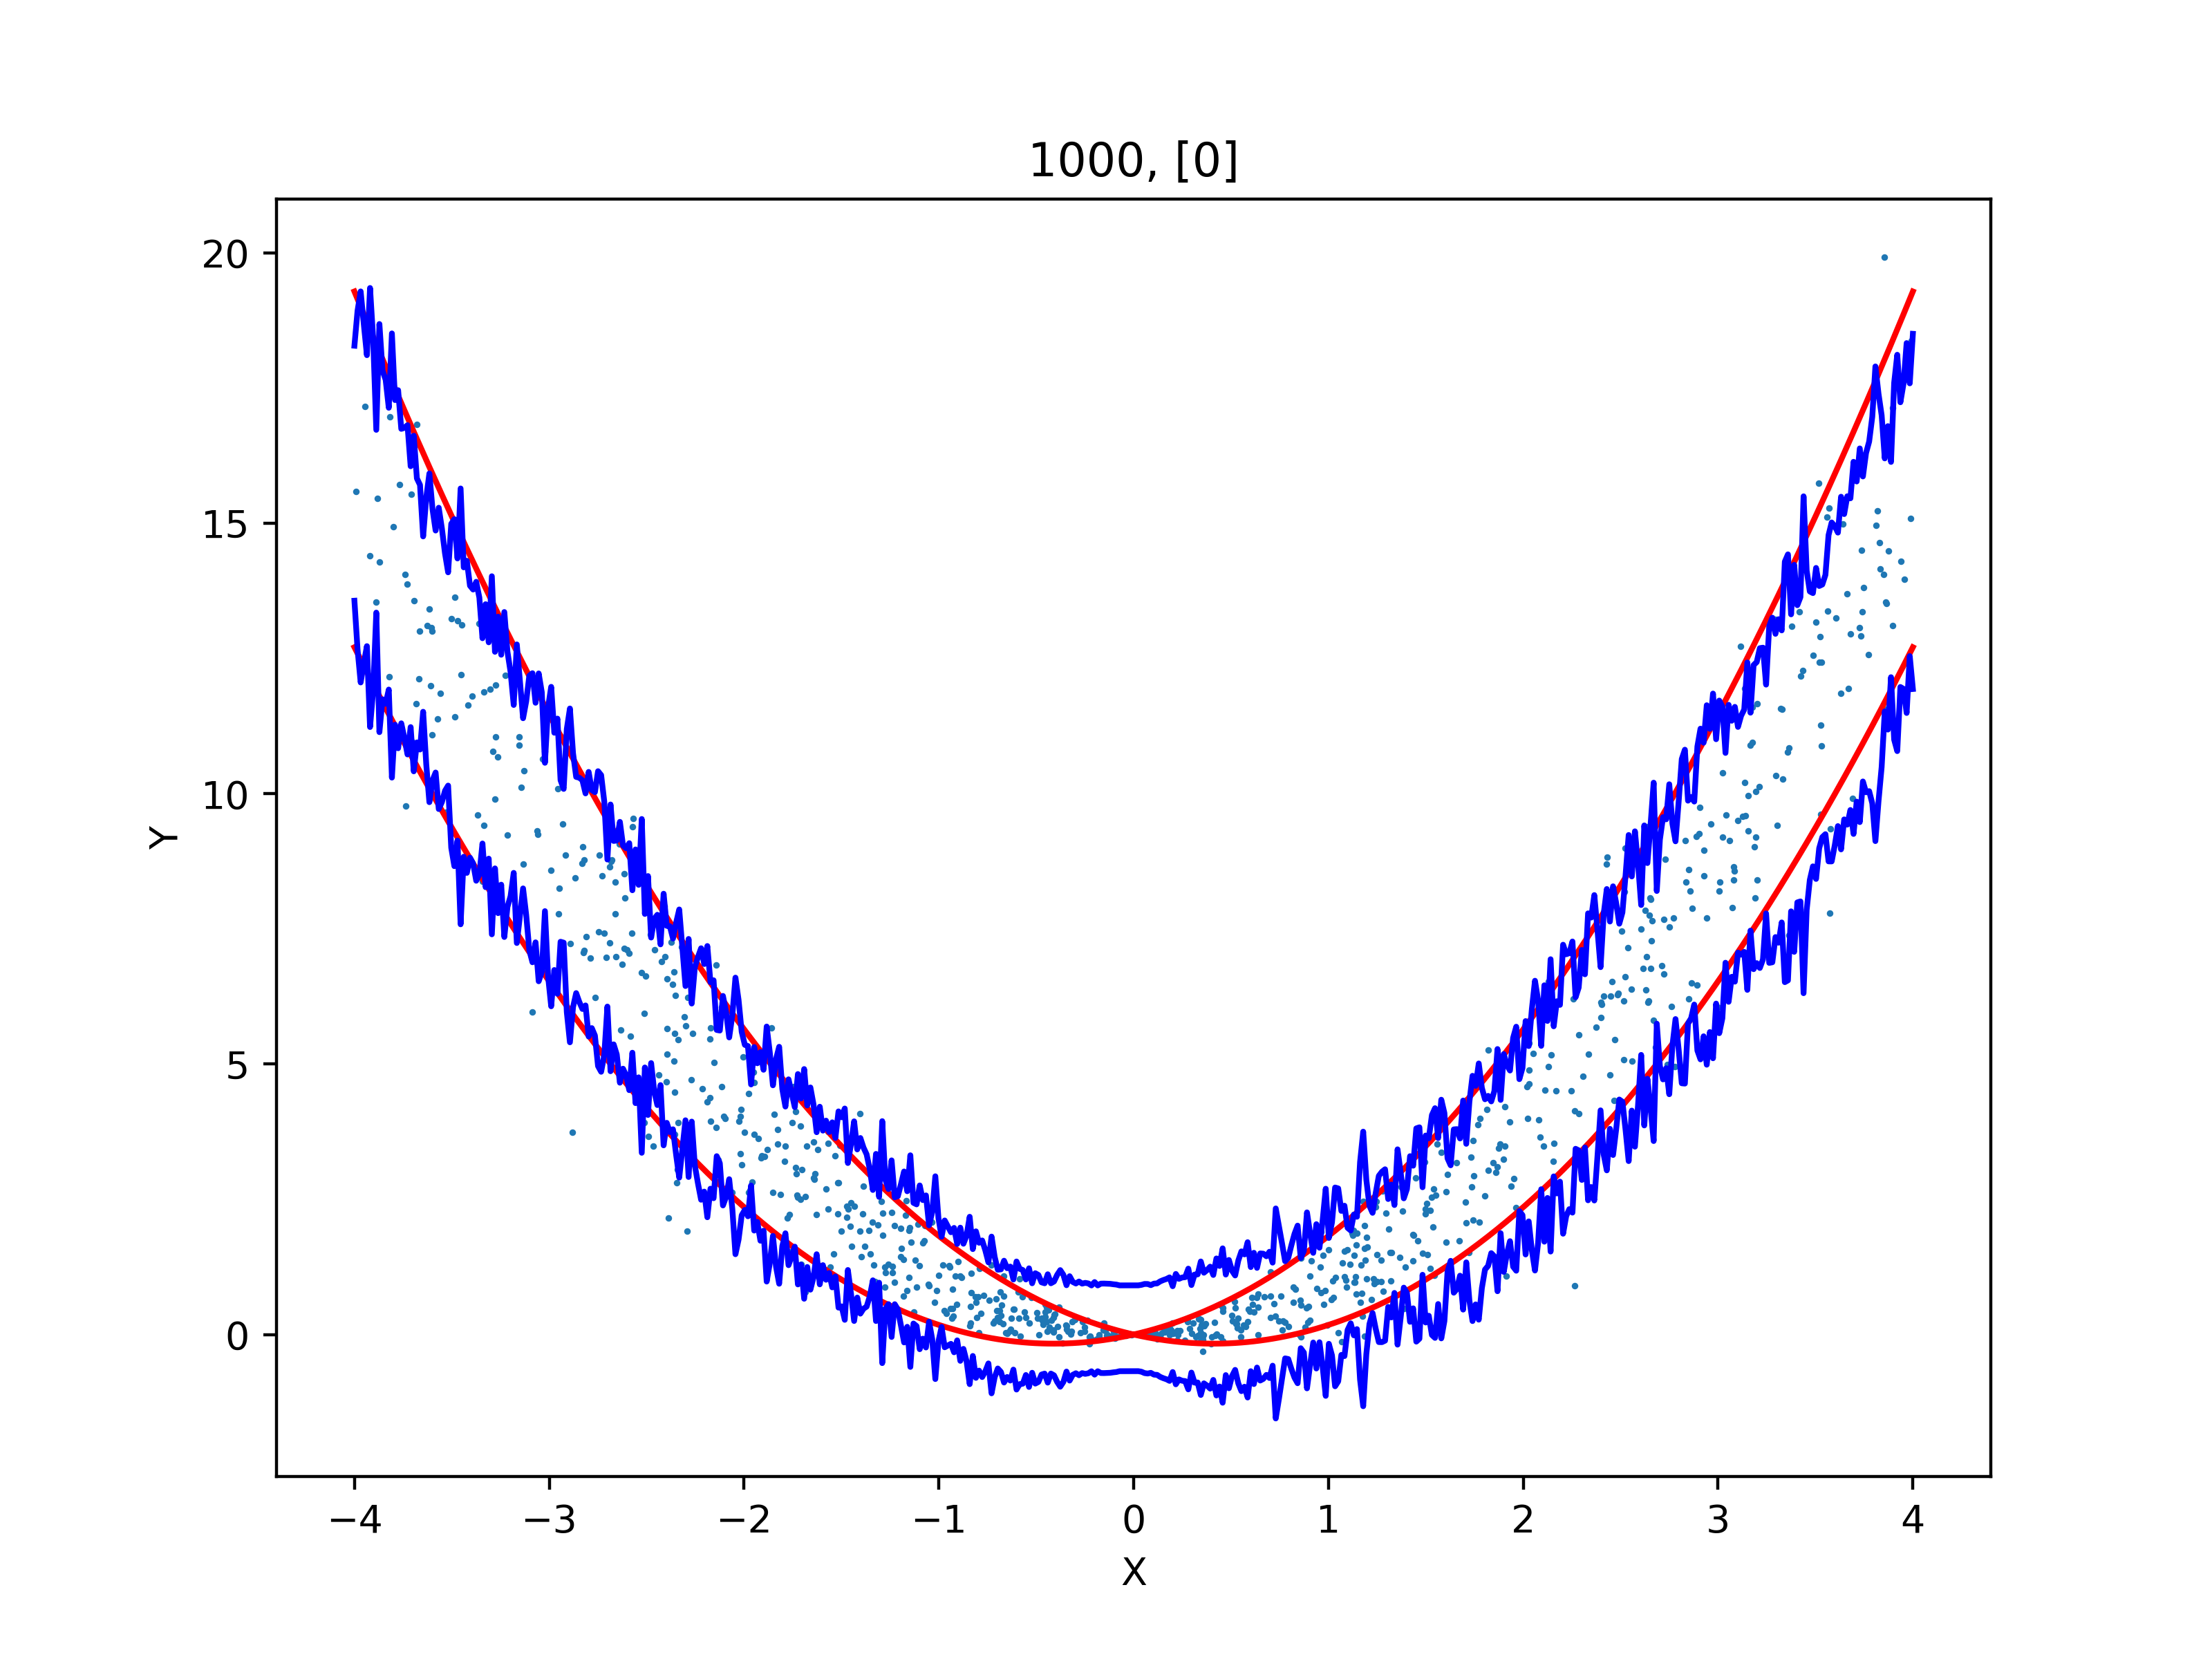
\includegraphics[width=0.98\linewidth]{fig/Ex1_1/0.png}
        \end{minipage}
        \begin{minipage}{0.495\linewidth}
            \centering
            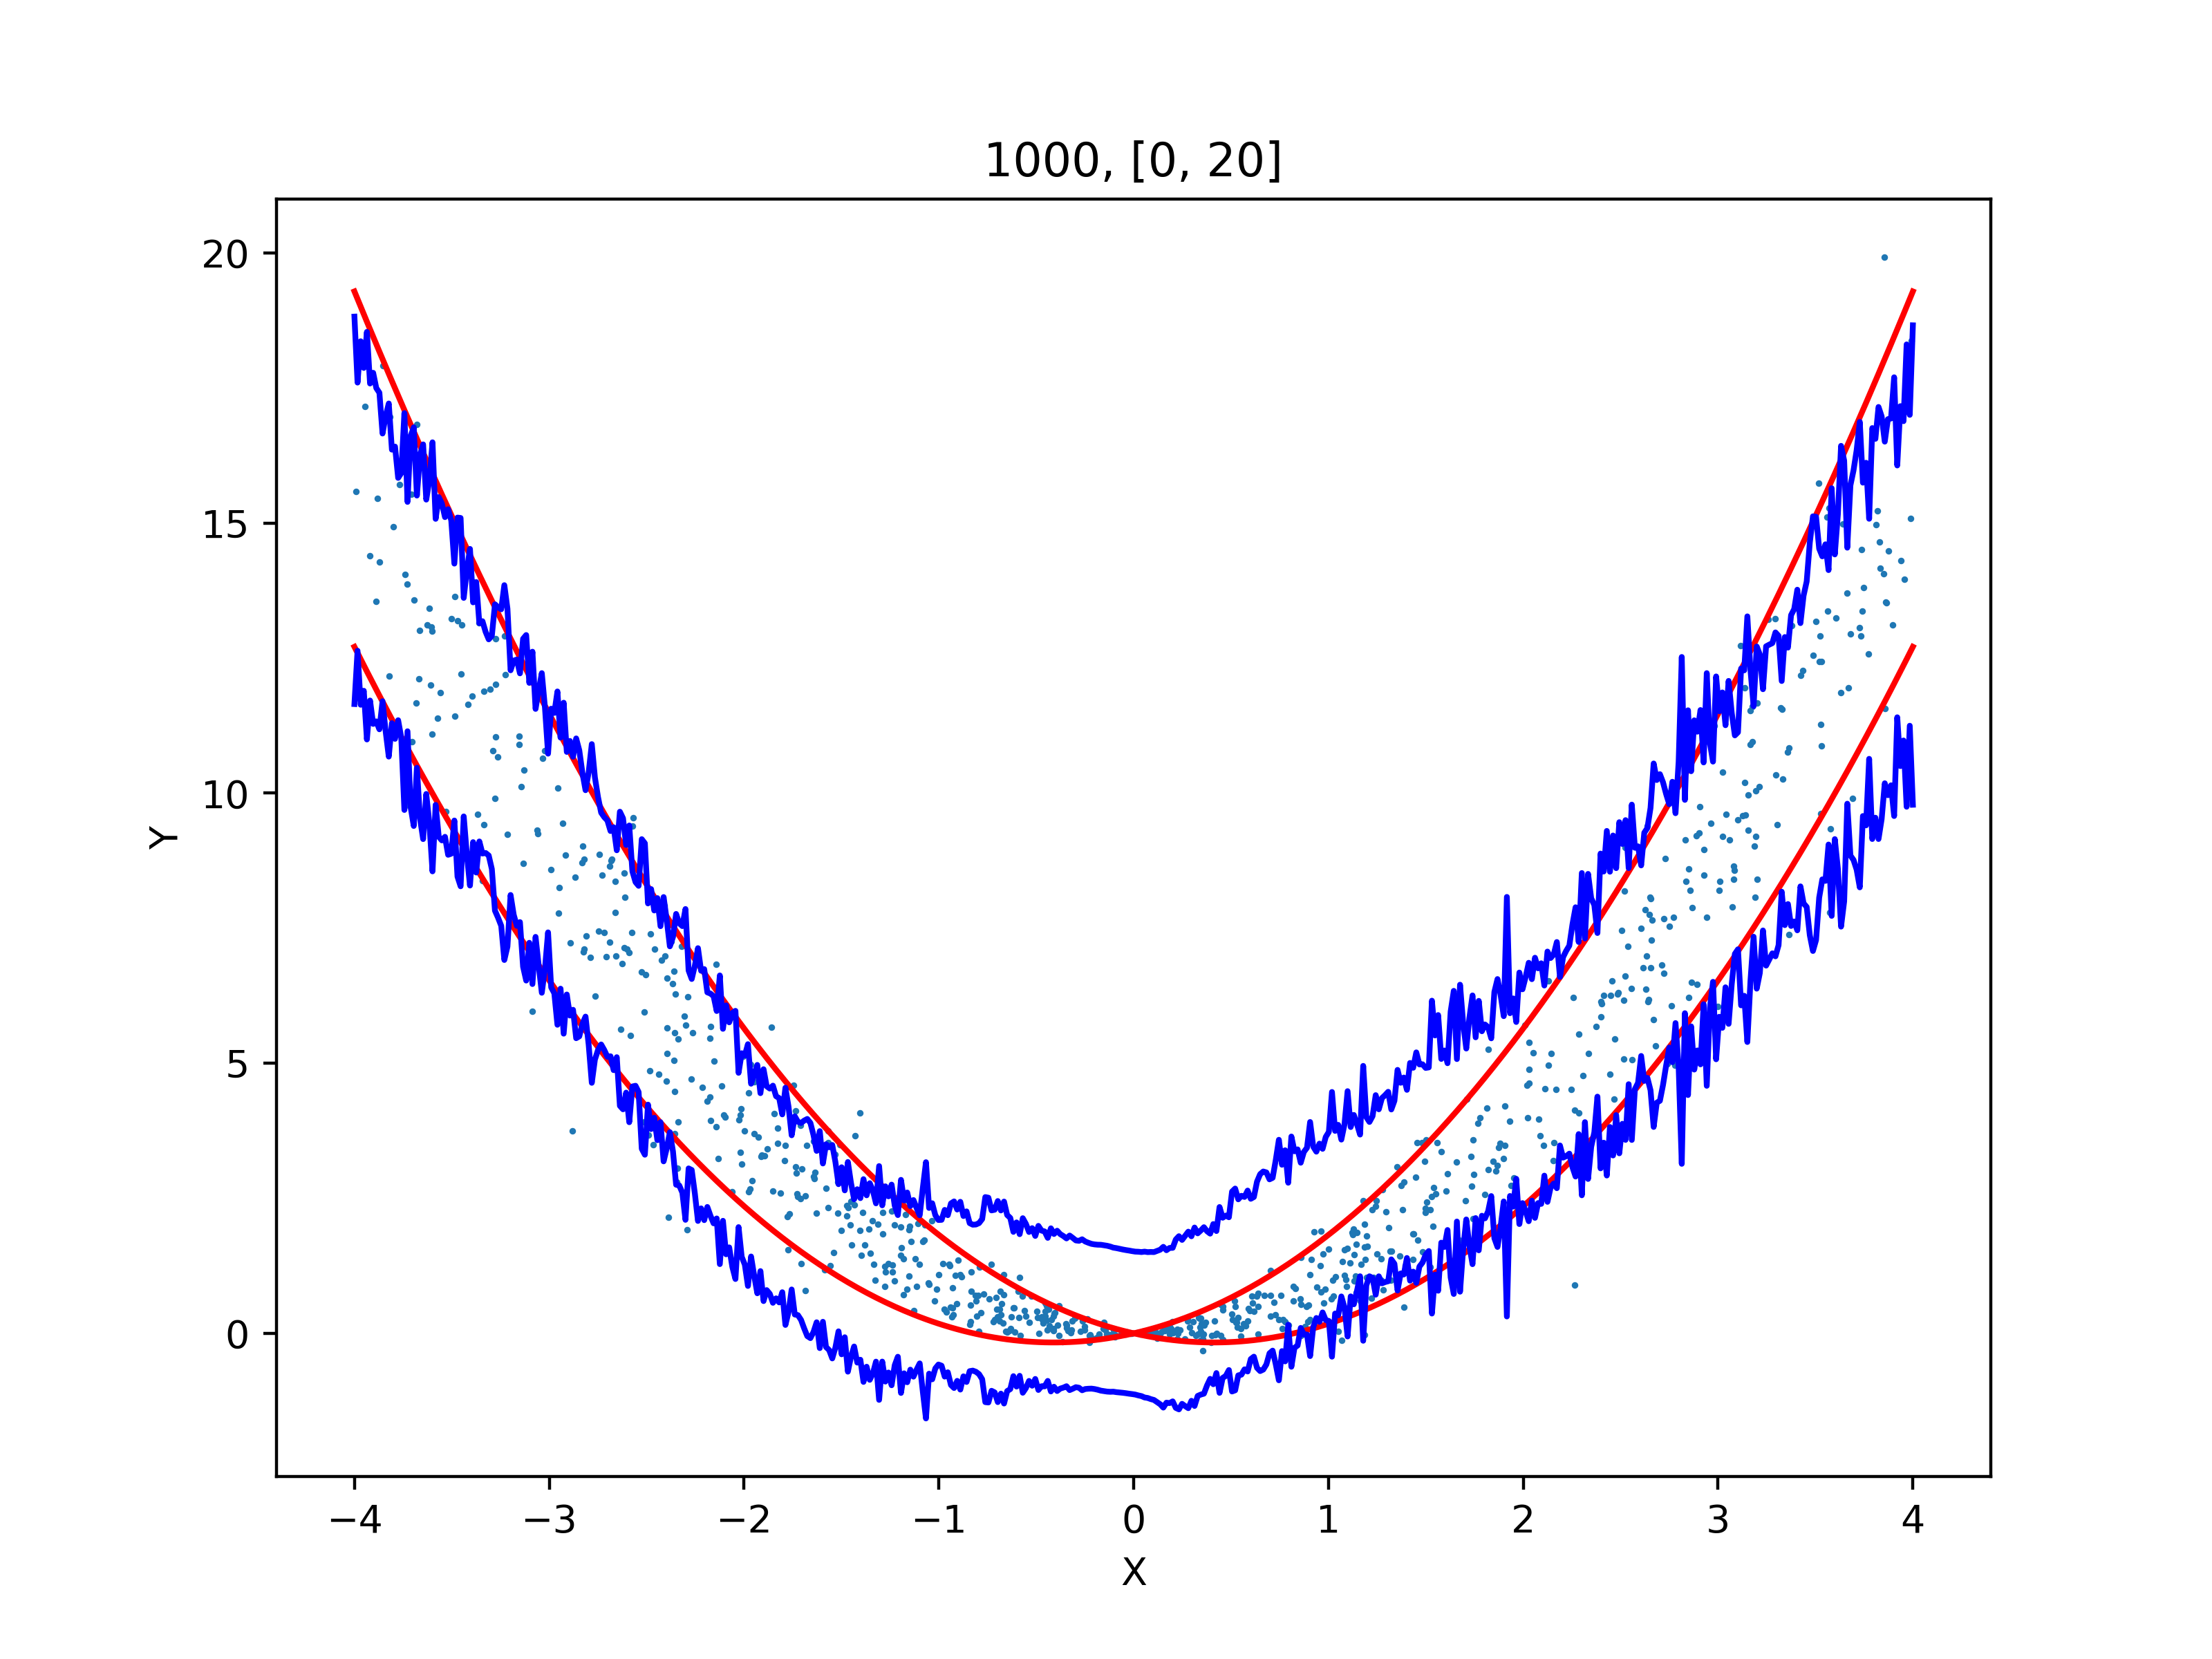
\includegraphics[width=0.98\linewidth]{fig/Ex1_1/0_20.png}
        \end{minipage}
        \caption{Fig2}
        \label{Fig2}
    \end{figure}

\subsection{Experiment2}
    Assume agent $k=1,\cdots,K$ each has $n$ samples $X_1^k,\cdots,X_n^k$ follow $N(\mu_k,9)$. Sythesize $Y_i^k=(X_i^k)^2+\epsilon$, where $\epsilon\sim N(0,(ep*|X|+ep*\theta_k)^2)$, $ep$ be some parameter and $\theta_k$ generated for each agent randomly between $1$ and $10$.
    \begin{itemize}
        \item $X$ has different distribution for each agents
        \item $EY|X$ is same for all agents
        \item $Y-EY|X$ has different distribution for different agents
    \end{itemize}
\newpage
\bibliographystyle{plain}
\bibliography{ref}
\end{document}